\subsection{同定と検証残差から見た補償の限界}

逆モデルやモデルベースフィードフォワードは、目標速度や既知外乱から必要入力を先に計算できるため、フィードバックだけに頼る場合より偏差を小さくできる。しかし、その計算はモデルを信じる操作でもある。DC モータ速度制御で
\begin{equation}
  \tau_n\dot{\omega}+\omega=K_n v
\end{equation}
という名目モデルを置くと、望ましい速度 $\omega_r(t)$ に対する単純な逆モデルフィードフォワードは
\begin{equation}
  v_{ff}(t)
  =
  \frac{\tau_n\dot{\omega}_r(t)+\omega_r(t)}{K_n}
  \label{eq:identified-inverse-feedforward}
\end{equation}
である。ここで $v$ は入力電圧 $[\mathrm{V}]$、$\omega$ は角速度 $[\mathrm{rad/s}]$、$K_n$ は定常ゲイン $[\mathrm{rad/s/V}]$、$\tau_n$ は時定数 $[\mathrm{s}]$ である。$K_n$ が実機より大きく見積もられていれば必要電圧は小さく計算され、加速不足が残る。$\tau_n$ が実機より小さければ、加速に必要な電圧を過小評価する。静止摩擦、デッドゾーン、負荷トルク、電圧飽和が入ると、式 \eqref{eq:identified-inverse-feedforward} の誤差はさらに大きくなる。

したがって、モデルベース補償を使う前に、実測データでモデルを同定し、別のデータで検証する必要がある。同定は「係数をもっともらしく決める」作業であり、検証は「その係数で、まだ見ていない運転条件をどの程度予測できるか」を測る作業である。補償の主張は、検証残差より細かくはならない。検証データで $1\,\mathrm{rad/s}$ 程度の予測誤差が残っているモデルを使って、フィードフォワードだけで $0.1\,\mathrm{rad/s}$ の追従精度を保証することはできない。

\subsubsection{同定用データと検証用データの分離}

まず、モータに複数の電圧レベルを与え、入力 $v_k$ と速度測定値 $\omega_k$ をサンプリング周期 $T_s$ ごとに記録する。電圧は正負の両側を含み、速度が上がる区間、下がる区間、低速でデッドゾーンの影響を受ける区間を含める。一定電圧を一つだけ入れたデータでは、時定数とゲイン、バイアス、摩擦を分けて読み取れない。

ここでは連続時間の一次モデル
\begin{equation}
  \tau\dot{\omega}+\omega=Kv+\omega_b
  \label{eq:identification-first-order-model}
\end{equation}
を、サンプル値の近似モデル
\begin{equation}
  \omega_{k+1}
  =
  a\omega_k+bv_k+c+\varepsilon_k
  \label{eq:identification-discrete-first-order}
\end{equation}
として当てはめる。$\varepsilon_k$ は、測定ノイズ、未測定外乱、モデルに入れていない摩擦やデッドゾーンの影響をまとめた残差である。式 \eqref{eq:identification-discrete-first-order} で $0<a<1$ なら、連続時間の時定数とゲインは
\begin{equation}
  \hat{\tau}
  =
  -\frac{T_s}{\log \hat{a}},
  \qquad
  \hat{K}
  =
  \frac{\hat{b}}{1-\hat{a}}
  \label{eq:identification-continuous-parameters}
\end{equation}
へ戻せる。$c$ は平衡点のずれや低速摩擦を一次モデルの中で吸収する項であり、理想的な線形モータでは 0 に近い。

同定では、データ全体を一度に使わず、前半を同定用、後半を検証用に分ける。時刻 $t_k$ が $0.4\,\mathrm{s}$ から $8.0\,\mathrm{s}$ までのサンプルを同定用集合 $\mathcal{D}_{id}$ とし、それ以降を検証用集合 $\mathcal{D}_{val}$ とする。各サンプルについて
\begin{equation}
  \phi_k=
  \begin{bmatrix}
    \omega_k\\
    v_k\\
    1
  \end{bmatrix},
  \qquad
  \theta=
  \begin{bmatrix}
    a\\
    b\\
    c
  \end{bmatrix}
\end{equation}
と置くと、予測式は $\omega_{k+1}=\phi_k^\T \theta+\varepsilon_k$ である。同定用データに対する二乗残差和
\begin{equation}
  J_{id}(\theta)
  =
  \sum_{k\in\mathcal{D}_{id}}
  \left(\omega_{k+1}-\phi_k^\T \theta\right)^2
  \label{eq:identification-least-squares-cost}
\end{equation}
を最小にする係数は、正規方程式から
\begin{align}
  0
  &=
  \frac{\partial J_{id}}{\partial \theta}
  =
  -2\sum_{k\in\mathcal{D}_{id}}
  \phi_k\left(\omega_{k+1}-\phi_k^\T \theta\right),\\
  \left(\sum_{k\in\mathcal{D}_{id}}\phi_k\phi_k^\T\right)\hat{\theta}
  &=
  \sum_{k\in\mathcal{D}_{id}}\phi_k\omega_{k+1},\\
  \hat{\theta}
  &=
  \left(\sum_{k\in\mathcal{D}_{id}}\phi_k\phi_k^\T\right)^{-1}
  \sum_{k\in\mathcal{D}_{id}}\phi_k\omega_{k+1}
  \label{eq:identification-normal-equation}
\end{align}
で与えられる。ただし、括弧内の行列が逆行列を持つには、入力と速度が十分に変化し、$\omega_k$、$v_k$、定数項の情報が同じ向きに偏りすぎていないことが必要である。

\begin{figure}[tbp]
\centering
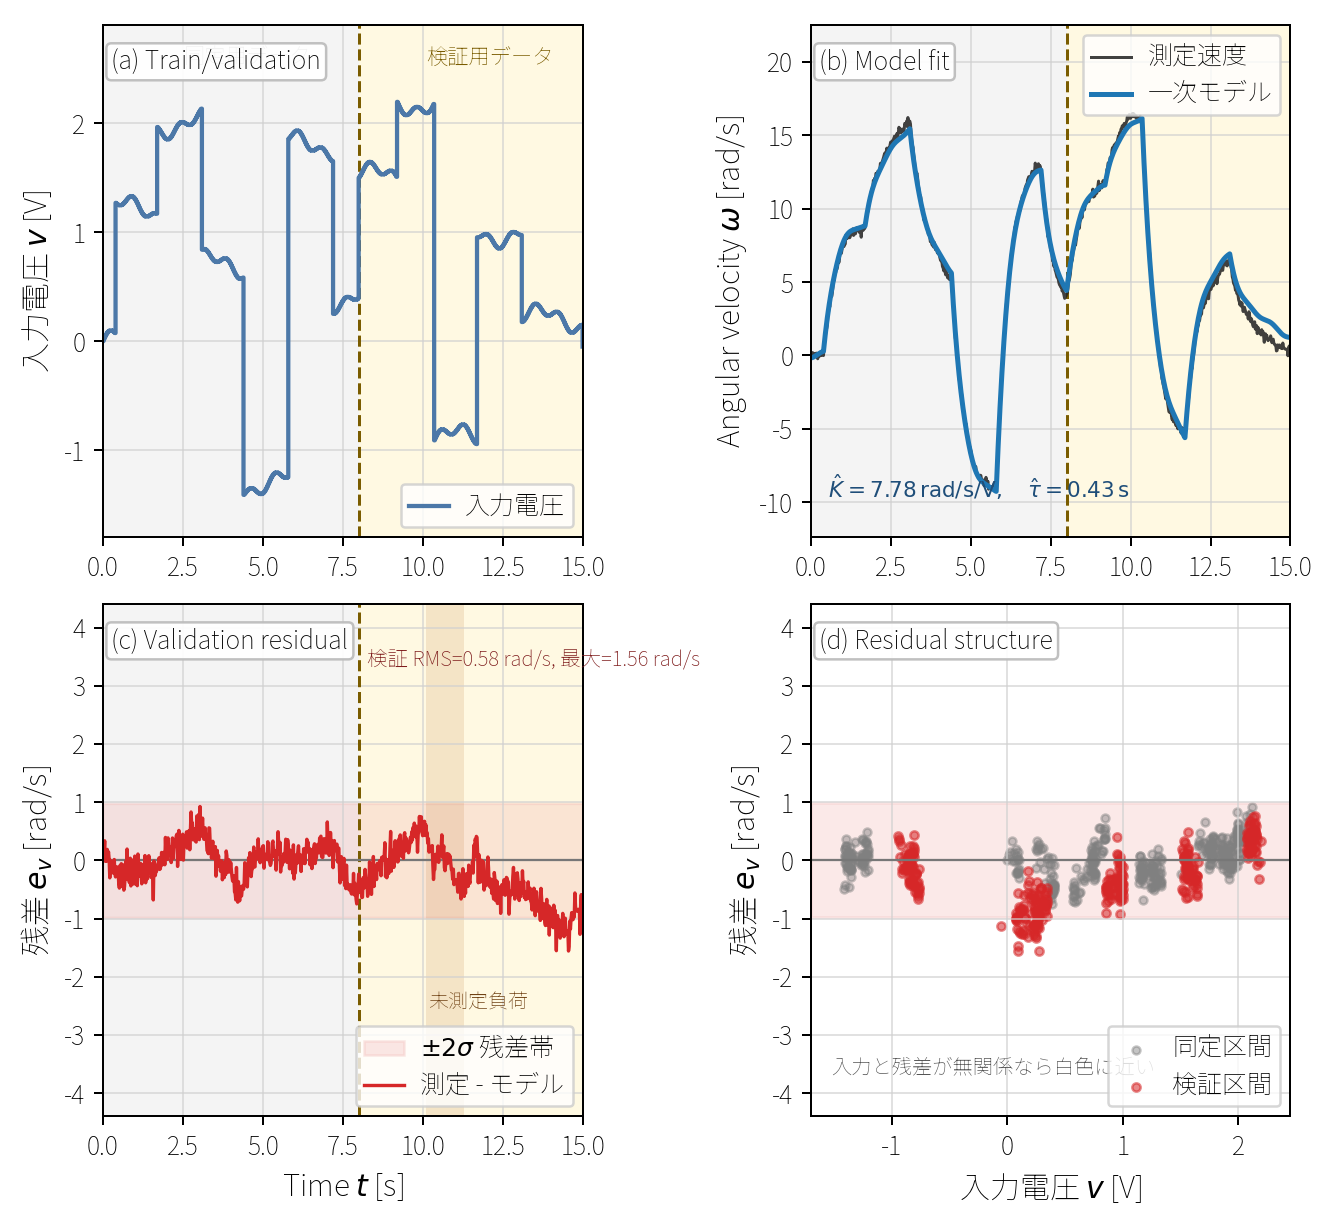
\includegraphics[width=0.98\linewidth,bb=0 0 1332 1224]{figures/identification_residual_examples.png}
\caption{DC モータ速度応答の一次モデル同定と検証残差。上段左は入力電圧の時系列で、灰色を同定用データ、淡い黄色を検証用データとした。上段右は同定用データから得た $\hat{K}=7.78\,\mathrm{rad/s/V}$、$\hat{\tau}=0.43\,\mathrm{s}$ の一次モデルを全区間へ適用した結果である。下段左は測定速度とモデル予測の差であり、検証区間の RMS 残差は $0.58\,\mathrm{rad/s}$、最大絶対残差は $1.56\,\mathrm{rad/s}$ である。下段右は入力電圧と残差の関係を表し、残差が入力や検証区間に依存している部分が未モデル化要素を表す。}
\label{fig:identification-residual-examples}
\end{figure}

\wfig{identification-residual-examples} は、サンプリング周期 $T_s=0.02\,\mathrm{s}$ で記録した速度データに、式 \eqref{eq:identification-discrete-first-order} を当てはめた例である。同定用データだけを見ると、測定速度とモデル速度はよく重なっている。推定値は $\hat{K}=7.78\,\mathrm{rad/s/V}$、$\hat{\tau}=0.43\,\mathrm{s}$ であり、少なくとも同じ範囲の電圧変化に対しては、一次遅れ近似として使える。

重要なのは、同定に使っていない検証区間で残差を読むことである。検証残差を
\begin{equation}
  e_{v,k}
  =
  \omega_k-\hat{\omega}_k
  \label{eq:validation-residual}
\end{equation}
と定義する。ここで $\hat{\omega}_k$ は、推定した係数を固定したまま、実際の入力電圧列を入れて計算したモデル速度である。図の検証区間では
\begin{equation}
  e_{rms}
  =
  \sqrt{
  \frac{1}{N_{val}}
  \sum_{k\in\mathcal{D}_{val}}e_{v,k}^2
  }
  =
  0.58\,\mathrm{rad/s},
  \qquad
  \max_{k\in\mathcal{D}_{val}}|e_{v,k}|
  =
  1.56\,\mathrm{rad/s}
  \label{eq:validation-residual-values}
\end{equation}
となっている。下段左の $10.1$ から $11.3\,\mathrm{s}$ 付近では、未測定負荷を入れたため残差が偏る。下段右では、検証区間の残差が入力電圧の値によってまとまっており、残差が単なる白色測定ノイズだけではないことが分かる。この構造は、デッドゾーン、速度依存ゲイン、負荷トルク、温度による抵抗変化などが一次モデルから漏れていることを意味する。

\subsubsection{残差がフィードフォワードの主張を制限する}

同定したモデルを式 \eqref{eq:identified-inverse-feedforward} に入れると、速度目標から電圧を先回り計算できる。しかし、検証残差が残っているなら、フィードフォワード後の誤差もその残差の範囲を基準に読まなければならない。一次モデルの予測誤差を連続時間で
\begin{equation}
  \tau\dot{\omega}+\omega=Kv+w_m(t)
  \label{eq:model-error-as-disturbance}
\end{equation}
と表すと、$w_m$ はモデル誤差を出力側へ換算した信号である。名目逆モデルで $v_{ff}$ を作っても、実機には
\begin{equation}
  \tau\dot{\omega}+\omega
  =
  K v_{ff}+w_m(t)
\end{equation}
が残る。$\tau$ と $K$ が名目値とずれ、さらに $w_m$ が検証残差として現れているなら、開ループのフィードフォワードだけではその成分を消せない。フィードバックは、この残差、未知外乱、初期値ずれを測定偏差として受け取り、安定余裕と入力制約の範囲で修正する役割を持つ。

残差は、補償の設計範囲を決める実験的な境界でもある。図の例では、同じ電圧範囲と同じ温度条件で検証したとき、RMS 残差は $0.58\,\mathrm{rad/s}$ である。したがって、このモデルを使った速度フィードフォワードは、少なくとも同程度の速度誤差が残る可能性を前提に置く。制御仕様として定常速度誤差を $0.2\,\mathrm{rad/s}$ 以下にしたいなら、一次モデルだけでは根拠が足りない。摩擦やデッドゾーンを別に同定する、負荷トルクを測る、フィードバック帯域を上げる、参照値を遅くして飽和を避ける、といった追加の根拠が必要になる。

また、残差がランダムに散らばらず、入力電圧、速度、回転方向、温度、時間に依存して偏る場合は、平均値を 0 に近づけただけでは不十分である。残差が入力電圧に依存しているなら、ゲインが一定でない。残差が速度の符号で変わるなら、摩擦やデッドゾーンが残っている。残差が特定時刻で偏るなら、未測定負荷や電源電圧の変動が入っている。残差が高周波に多いなら、センサノイズやサンプリング遅れを逆モデルが増幅している。これらの構造を見ずに、二乗誤差の平均だけで「モデルはよい」と判断すると、補償が効く範囲を過大評価する。

\subsubsection{補償後に残るロバスト性限界}

ここまでの流れでは、飽和に対してアンチワインドアップを入れ、参照値を整形し、カスケード制御で内部量を速く制御し、摩擦やデッドゾーンを補償し、さらにモデルベースフィードフォワードで必要入力を先に与えた。それでも制御系が完全になるわけではない。残る限界は、少なくとも次の五つに分けられる。

第一に、モデル誤差である。同定した一次モデルは、同定データの範囲で平均的に合う近似であり、すべての速度、温度、負荷、電源電圧、摩耗状態で正しい物理式ではない。検証残差が入力や時刻に依存しているなら、その依存性はフィードフォワード後にも残る。必要なら、速度依存ゲイン、摩擦項、デッドゾーン、むだ時間、電圧飽和をモデルに加え、追加した項ごとに別の検証データで残差が本当に減ったかを確認する。

第二に、未測定外乱である。負荷トルクや路面抵抗が測定できる場合は外乱フィードフォワードで先に補える。しかし、測れていない外乱、遅れて届く外乱、符号や単位がずれた外乱は残差として現れる。外乱補償の効果は、外乱測定の帯域、遅れ、ノイズ、取り付け位置に制限される。

第三に、測定ノイズである。同定ではノイズが係数推定を揺らし、検証では残差の下限を作る。逆モデルや微分を含むフィードフォワードは高周波ノイズを大きくしやすい。したがって、速度や加速度を使う補償では、フィルタの遅れとノイズ低減を同時に見なければならない。ノイズを完全に消そうとしてフィルタを遅くしすぎると、今度は補償入力が実際の運動から遅れる。

第四に、飽和とレート制限である。モデルが正しくても、式 \eqref{eq:identified-inverse-feedforward} が電圧、電流、トルク、速度、温度の制約を越える入力を出すなら、その入力は実機へ入らない。飽和後の入力で動く実機は、同定に使った線形モデルとは別の非線形系になる。したがって、同定残差が小さいことと、要求入力が実現可能であることは別々に確認する必要がある。

第五に、推定値の不確かさである。$\hat{K}$ と $\hat{\tau}$ は有限のデータから得た値であり、入力波形、測定ノイズ、サンプリング周期、運転条件に依存する。別の日、別の温度、別の負荷では推定値が変わる。実装では、係数を一点の値として扱うだけでなく、検証残差と係数のばらつきから余裕を残す。たとえば、フィードフォワード入力を少し控えめにし、フィードバックで残差を吸収し、残差が増えたときには補償を弱める監視を入れる。

この段階で得られる結論は、モデルベース補償を捨てることではない。むしろ、モデルを使う範囲を実測で区切ることで、フィードフォワードとフィードバックの役割分担が明確になる。フィードフォワードは、検証された帯域と入力範囲で既知の運動や既知外乱を先に補う。フィードバックは、検証残差、未知外乱、ノイズ、飽和、係数ずれを受け止める。次に性能指標を導入するときは、追従誤差だけでなく、RMS 入力、ピーク入力、制約余裕、残差の大きさを同時に数値化し、手調整でどこまで改善でき、どこから複数目的の重み付けが必要になるかを評価する。
